\documentclass{article}
\usepackage[utf8]{inputenc}
\usepackage{amsmath}
\usepackage{graphicx}
\usepackage[colorinlistoftodos]{todonotes}
\usepackage{hyperref}
\usepackage{enumitem}
\usepackage{lipsum}% for dummy text
\usepackage{exercise}
\usepackage{epigraph}
\usepackage{dirtytalk}
\usepackage[ruled,vlined]{algorithm2e}


\title{Bayesian Statistics: A Summer Term Primer \\
\large Getting the Most From Data}
\author{Jesse Galdal-Gibbs}
\date{2020/21}

\begin{document}
\maketitle

\begin{abstract} Draft.
Some theory, examples, problems and code for Y13s in lockdown.
\end{abstract}

\epigraph{I know loads of people who've had coronavirus. They didn't take the test but had the symptoms.}{\textit{Lots of my friends \\ Varied educational backgrounds}}

\section{Prerequisites}
All you need is knowledge of the conditional probability formula, integration of polynomials and exponentials, summation and product notation, and a willingness to Google (when you need to code something new to you). If we get on to MCMC, having taken the Markov Chain course may help.

\section{Introduction}

Suppose 20 patients are admitted to hospital and test positive for SARS-CoV-2. They have been sent to particular hospitals by coordinated NHS contact-aware systems so that they can be considered to be independent of each other; they are neither relatives nor neighbours nor have anything in common that any group wouldn't have. Some of these people will recover at this stage, but others will go on to need intensive care.

\begin{enumerate}[leftmargin=2cm,labelsep=0cm,align=left,label={[\arabic*]}]
    \item How many will go to ICU?
    \item How likely is it that most of them go to ICU?
    \item How should I incorporate new information into my model as patients' conditions develop?
\end{enumerate}

We could model the number of these patients needing to go to ICU as following a Binomial distribution with parameters (sample size, probability of a patient's needing ICU) being (20, $\theta$) respectively. In the Frequentist, or Classical, paradigm, we would treat $\theta$ as an unknown constant. Inference would include using Maximum Likelihood Estimators to find the $\theta$ most consistent with observations and finding Confidence Intervals for $\theta$. It would exclude statements like \say{the probability that $\theta$ is more than 25\% is 50\%.} The Classicist treats $\theta$ as a point, the Bayesian as a curve.

There is plenty of literature on Bayesian methods and the paradigm, including computer-based methods; I can recommend many free MOOCs and similar. Here I compile a few results that are essential and accessible in the space allocated. It is of course far from comprehensive, but I hope will whet your appetite; and, if you do not go on to study this in more detail, I hope it provides some tools for evaluating claims and data in everyday life.

\paragraph{Using this Resource}
To simulate in-person lesson, there are preparatory exercises where I felt it appropriate that the student discover the next piece of theory through active reading, and consolidation exercises for practising techniques seen in the notes.


As another motivating example, consider the case of Sally Clark, wrongly jailed after losing two children to SIDS.\footnote{Sally Clark Wikipedia \url{https://en.wikipedia.org/wiki/Sally_Clark}.} Besides the flaws in statistical evidence leading to her conviction - including treating the two children's deaths as statistically independent, rather than considering the necessary similarities in genetic and environmental factors - it is interesting to note that the statistical logic behind the initially successful prosecution case went something like:
\begin{enumerate}[leftmargin=2cm,labelsep=0cm,align=left,label={[\arabic*]}]
   \item suppose she is innocent;
   \item what are the chances of the observed deaths?
   \item low;
   \item hence reject the supposition and conclude she is guilty.
\end{enumerate}
In other words, the probability being considered is the probability of the deaths given she is innocent, or
\begin{equation}
{p(\text{data}|\text{hypothesis})}.    
\end{equation}

\begin{Exercise}
    What would our judicial system have to say about whether someone had cheated or not when they win the lottery? Generalise.
\end{Exercise}
\vspace{5mm}

Here we begin to spot how the Bayesian paradigm differs from the classical one. Firstly they ask different questions: the Classicist sees something weird and, wondering if their null hypothesis holds up, ask \say{what were the chances of that?}. A Bayesian gathers data and asks \say{what is the probability of my hypothesis given the data}. It can be considered an iteration as new data come in. Many feel that the Bayesian question is the right one to ask; it is certainly more intuitive for most people.

A second difference is in treatment of parameters. Where the Classicist considers the object of consideration to be an unknown constant, the Bayesian considers it a variable with a probability distribution. The former creates probability intervals which are statements about limiting behaviour in repeated sampling, while the latter creates a credibility interval which is the probability that the parameter is in that interval. It is what students think a probability interval is until we teachers bash that prose (\say{the probability that, on long-term repeated sampling, an interval created this way would contain the parameter}) into them, while wishing we could just stick to the intuition-friendly approach of Bayes.

In practice the Bayesian approach is best suited for small data sets crunched with big computers, which is quite a niche. To elaborate, it is more necessary the smaller the data set, and more tractable the bigger the computer. This is because most functions cannot be integrated analytically and so numerical methods are used (see MCMC below).

Bayes' Formula exists in many forms. Central to all of them is the idea of starting with a subjective probability (/density function) in advance of gathering data, known as the \textbf{prior}; adding data to ones knowledge, and forming an improved model combining what one thought with what one sees, called the \textbf{posterior}. In the SARS-CoV-2 example, the expert in charge chooses a subjective distribution of $\theta$ based on prior knowledge of similar diseases; it will be some curve between zero and one, usually with a peak somewhere and values for mean and variance which are all generally consistent with similar diseases. This distribution is the \textbf{prior}, written $f(\theta)$. As patients recover or get transferred to ICU, this data changes the distribution into the \textbf{posterior}, written $f(\theta|data)$. If the observed transfer rate in the data is much higher than with previous diseases that informed the choice of prior, then the mean will shift to the right and this will show in the posterior. The distribution of the observable variable - the number of patients going to ICU - is known as the \textbf{likelihood}, and in our example is given by the Binomial probability formula

\begin{equation}
    f(x|\theta) = \binom{20}{x}  \theta^x (1-\theta)^{20-x}. \label{Binomial_20}
\end{equation}

Before quoting the formula in its most useful forms, note how the Conditional Probability formula can be expressed as

\begin{equation}
\begin{split}
        p(A|B)
        &=\frac{p(A\cap B)}{p(B)} \\
        &=\frac{p(B|A)p(A)}{p(B)}. \label{BayesVanilla}
\end{split}
\end{equation}

\newpage

This is essentially Bayes' Formula. Note also that the denominator is usually found through calculation rather than provided, and done so by averaging over all the values A can take. These are the discrete and continuous versions, respectively:

\begin{equation}
    p(B)=\Sigma_A \ p(B|A)p(A) \ \text{and}
\end{equation}

\begin{equation}
    p(B)=\int_A \ p(B|A)p(A) \ dA \label{normalising_constant}
\end{equation}

The most useful forms of Bayes' Formula for our discussion refer to hypotheses (or parameters) and data:

\begin{equation}
    {p(hyp|data)=p(data|hyp)\frac{p(hyp)}{p(data)}};
\end{equation}

\begin{equation}
    posterior = prior \times odds; 
\end{equation}

\begin{equation}
    posterior = \frac{likelihood \times prior}{normalising \; constant} \text{\ ; and}
\end{equation}

\begin{equation}
    posterior \propto likelihood \times prior.
\end{equation}

\vspace{5mm}

To address the issue in the epigraph, note that we can rephrase the statement as \say{the probability that someone has coronavirus given they have the symptoms is large}. Without getting into a meaningful level of medical detail, we can see just how sensitive this claim is to adjustments in assumptions. Using Bayes' rule we can analyse the probability, defining $c$ as having coronavirus and $s$ as having the symptoms, as

\begin{equation}
    p(c|s)=\frac{p(s|c)p(c)}{p(s)}.
\end{equation}

We can then run a scenario analysis. Let's suppose $1\%$ of the population has the disease, and simultaneously pull the other two levers: how many young people with the virus have symptoms and how often they would have fever anyway (eg from the flu). Let's first assume everyone with the virus shows the symptoms (which is an overestimate) and that the demographic gets fever just under $1\%$ of the time (I have no idea if this is realistic). Then 

\begin{equation}
    p(c|s)=\frac{1 \frac{1}{100}}{\frac{1}{99}}=\frac{99}{100},
\end{equation}

suggesting these claims are correct. However, if the prevalence of fever were to increase to one in fifty, and the young demographic's propensity to display symptoms at a given instant of their infection turned out to be closer to a half, then we would see

\begin{equation}
    p(c|s)=\frac{\frac{1}{2}\frac{1}{100}}{\frac{1}{50}}=\frac{1}{4},
\end{equation}

which would tell a very different story. I am not taking a stance on the answer, just drawing your attention to a mechanism of looking for one.

\begin{Exercise}
    Share similar examples of everyday claims that could be analysed in this way with the rest of the class.
\end{Exercise}


\section{Informativeness of Data}

\begin{Exercise}
    \paragraph{An old chestnut but tricky}
    Solve the Monty Hall problem using a Bayesian rule:
    \say{Suppose you're on a game show, and you're given the choice of three doors: Behind one door is a car; behind the others, goats. You pick a door, say door A, and the host, who knows what's behind the doors, opens another door, say door B, which has a goat. He then says to you, "Do you want to pick door C?" Is it to your advantage to switch your choice?}
    
    \paragraph{Hint}
    The most difficult step is identifying the 'events' in the Bayesian formula, say in form \eqref{BayesVanilla}. Draw a three-step Tree Diagram.
\end{Exercise}

\begin{Exercise}
\paragraph{Preparatory Exercise}
Compare the impact of a positive test (screen) result in the following situations. Suppose for both the screen misses the disease 10\% of the time and gives a false alarm for 30\% of the uninfected. In country A the prevalence is 1 in 10,000 and B 1 in 100. Given a positive result, what is the probability of having the disease, and how much does this differ from the prevalence?

What about if the test were much better, and only gave incorrect readings 1\% of the time (for both the infected and uninfected)? 

Note how the positive test result is more informative in some circumstances than others. Why?
\end{Exercise}



\section{Hypothesis Comparison}
\begin{Exercise}
\paragraph{Preparatory Exercise}
I pick someone from either country above with equal probability. Given they have the disease, what are the chances they came from country A and B respectively? I suggest you write down your guess before you calculate the answer.
\end{Exercise}

\section{Continuous Parameters}
The discrete form of Bayes' formula in terms of data and hypothesis is

\begin{align}
\displaystyle p(H|d)= \frac{p(d|H)p(H)}{p(d)} 
= \frac{p(d|H)p(H)}{\sum_H {p(d|H)p(H)}}.
\end{align}


I have  chosen $d$ to denote data and $H$ hypothesis. Note how the $p$ appears in front of each argument and means a different thing depending on the argument. In the continuous case (see below), $p$ is replaced with $f$ by convention, which refers to the density function of the respective argument(s). At first it may take some forehead-wrinkling to remember that the different uses of $f$ are not generally the same function. $f(x)$ is the density function of $x$, which may follow a Normal distribution, while $f(y)$ is that of $y$, which may follow an Inverse Gamma distribution, say. We illustrate the continuous version with an example.

\subsection{Unfair Funfair Coin}
You are in a fairground and a game consists in your paying a non-negligible up front fee and either receiving lots of money or losing it (the amounts are irrelevant to this discussion - we are not currently studying maximising expected gain, but rather how data affect your distribution for the coin parameter). Defining $\theta$ as above (the chance of Heads on a flip), and noting that we have such little trust in the fairness of the game that the coin may be double-Heads, double-Tails, fair, or anything between, with nothing to separate this continuum of scenarios, we must first choose a prior distribution for $\theta$. The likelihood is given in equation \eqref{Binomial_20}.

Now $\theta$ is the continuous parameter. Remember, $\theta$ is a random variable, not an unknown constant.

\begin{align}
f(\theta|d) = \frac{f(d|\theta)f(\theta)}{f(d)}
= \frac{f(d|\theta)f(\theta)}{\int_{\theta} f(d|\theta)f(\theta)d\theta}.
\end{align}

It is already getting a bit 'meta' in that $f(\theta)$ is an expression of the probability of $\theta$'s being in a certain range, but $\theta$ itself is a probability. So that $f$ is the probability about a probability, in the coin example. But more generally, the parameter might be $\mu$, the mean height of a Year 13 pupil, or $\lambda$, the average number of times someone learning Python googles something in a ten-minute interval. Part of the power of the approach is it allows equal treatment of tangible quantities and probabilities.

\paragraph{Prior}
We choose the uninformative prior: the Uniform distribution on [0,1], so that 
\begin{equation}
    f(\theta)=1.
\end{equation}

\begin{figure}[h]
\centering
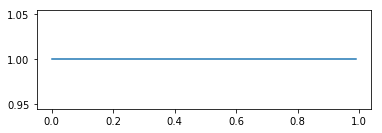
\includegraphics[width=0.3\textwidth]{1_unif.png}
\caption{\label{fig:frog}Uninformative prior: PDF $f(\theta)$ against $\theta$}
\end{figure}

\paragraph{First flip: Heads}

Suppose we then flip the coin and get Head. We then perform the Bayesian update to get a posterior for theta given this new information. Then 
\begin{align}
f(\theta|{Head}) = \frac{f({Head}|\theta)f(\theta)}{f({Head})}
= \frac{f({Head}|\theta)f(\theta)}{\int_{\theta} f({Head}|\theta)f(\theta) d\theta}.
\end{align}

The likelihood, the probability of Head for a given $\theta$, is of course just $\theta$ (Bernoulli). The prior being 1 gives:
\begin{equation}
\begin{split}
f(\theta|{Head})
&= \frac{\theta}{\int_0^1 \theta} \\
&=\frac{\theta}{[\frac{1}{2}\theta^2]_0^1} \\
&=\frac{\theta}{\frac{1}{2}} \\
&= 2\theta
\end{split}
\end{equation}

This says that we are generally in favour of the coin having a Heads bias; it is impossible the coin is double-Tailed (zero density at $\theta=0$); the chance that the coin is roughly fair hasn't changed (see credibility intervals below).

\begin{figure}[h]
\centering
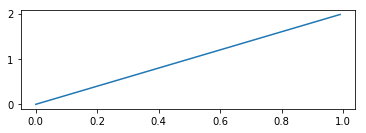
\includegraphics[width=0.3\textwidth]{2_H.png}
\caption{\label{fig:H} $f(\theta|\text{Head})$ vs $\theta$}
\end{figure}

\paragraph{Second flip: also Heads}
Now the sequence looks like {prior, Head, Head}. So we expect a flattening around $\theta=0$ in favour of more probability towards $\theta=1$. But on such a small sample we also expect the curve to continue to be consistent with the coin being fair. Iterating from this point, out previous posterior becomes our current prior; the likelihood is unchanged.

\begin{equation}
\begin{split}
f(\theta|{Head})
&= \frac{\theta \times 2\theta}{\int_0^1 \theta \times 2\theta \ d\theta} \\
&= 3\theta^2
\end{split}
\end{equation}

\begin{figure}[h]
\centering
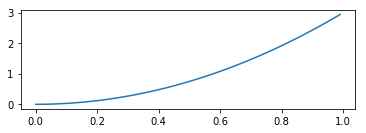
\includegraphics[width=0.3\textwidth]{3_HH.png}
\caption{\label{fig:HH} $f(\theta|\text{Head, Head})$ vs $\theta$}
\end{figure}

\paragraph{Third flip: Tails}
So far there remained a possibility that the coin was double-Headed; it got more plausible with each flip. That possibility has now been removed, and so the current distribution must have roots at both 0 and 1. A quick calculation confirms this; the likelihood is now the change of Tails, which is $1 - \theta$.

\begin{equation}
\begin{split}
f(\theta|{Tail})
&= \frac{(1-\theta) \times 3\theta^2}{\int_0^1 (1-\theta) \times 3\theta^2 \ d\theta} \\
&= 12(1-\theta)\theta^2
\end{split}
\end{equation}

\begin{figure}[h]
\centering
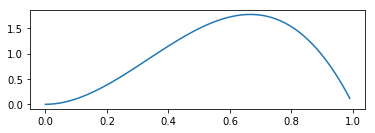
\includegraphics[width=0.3\textwidth]{4_HHT.png}
\caption{\label{fig:HHT} $f(\theta|\text{Head, Head, Tail})$ vs $\theta$}
\end{figure}

See the github\footnote{My github \url{https://github.com/jessesebastiangg/Bayes_sims}.} for interactive simulation.

\begin{Exercise}
\paragraph{Open exercise}
    Prove that in the above case the posterior arrived at is the same observing all three flips simultaneously and performing the update in one iteration.
    Prove, further, that this generalises.
\end{Exercise}

\newpage{}

\section{Conjugate Priors and Integration-Dodging}
You will have noticed that the numerator provided the information about shape, while the denominator is the definite integral of the numerator. It simply serves to guarantee that the function is a probability distribution, in particular that it integrates to 1. Think of finding a unit vector in a given direction.

This suggests a wonderful approach of "integration by spotting something is a known distribution".

NB the mathematical convenience of this approach should suggest to you (if something seems to good to be true then it probably is) that it means it is next to useless. Or perhaps worse than useless because it may encourage statisticians to choose these priors when they do not fit the world. Nonetheless it is nice.

The argument goes, using equation 4 above, that if the product of the likelihood with the prior form a recognised probability distribution up to proportionality, then the normalising constant must be the one in said form. This is best seen with examples.

The parameters of the parameter's distribution are known as \textbf{hyperparameters}. These could, of course, themselves be considered to be random variables following a distribution with yet more parameters, and so on, but I have yet to come across terms like \say{hyperhyperparameter} used seriously.

\subsection{Binomial Likelihood with Beta Prior/Posterior}
You may have noticed the distributions of $\theta$ at each iteration looked similar to each other, and indeed Binomial-ish. It turns out the Uniform distribution is a special case of the Beta distribution, which is like a theoretical (continuous) counterpart of the evidential Binomial distribution.

\subsubsection{The Beta Distribution}
The graphs above are all examples. It takes two parameters and is given by the following form:

\begin{equation}
    f(\theta)=\frac{\theta^ {\alpha-1} (1-\theta)^ {\beta-1}}{B(\alpha,\beta)}
    =\frac{\Gamma(\alpha+\beta)}{\Gamma(\alpha)\Gamma(\beta)}\theta^ {\alpha-1} (1-\theta)^ {\beta-1},
\end{equation}
where $B(\alpha,\beta)=\frac{\Gamma(\alpha)\Gamma(\beta)}{\Gamma(\alpha+\beta)}$, and the gamma function extends the factorial function beyond the natural numbers, coinciding as $\Gamma(n)=(n-1)!$. The Beta distribution has mean $\frac{\alpha}{\alpha+\beta}$, reinforcing the notion that $\alpha$ is a counterpart to x in the Binomial, ie the number of successes, and $\beta$ the number of failures. 


\subsubsection{Conjugacy}
A prior distribution is said to be conjugate to a likelihood if the posterior takes the same form as the prior. For example, for a Binomial likelihood, any Beta prior results in a Beta posterior. To prove the Beta-Binomial (or -Bernoulli) conjugacy, note that our claim is that if the prior distribution for $\theta$ is Beta($\alpha,\beta$), and the likelihood Binomial(n,$\theta$), then the posterior is Beta($\alpha',\beta'$) for some new parameters $\alpha',\beta'$, which we will find. This will provide a shortcut for the update procedure.

The posterior is found below. Note the omission of counting constants from both sides of the fraction, which would either both be the Binomial ones or 1 if a sequence of iid Bernoulli.

\begin{equation}
\begin{split}
f(\theta|x)
&= \frac{f(x|\theta)f(\theta)}{\int_0^1 f(x|\theta)f(\theta)\ d\theta} \\
&= \frac{\theta^x (1-\theta)^{n-x} \times \theta^{\alpha-1} (1-\theta)^{\beta-1}}{\int_0^1 numerator \space \ d\theta} \\
&= \frac{\theta^{\alpha+x-1} (1-\theta)^{\beta+n-x-1}}{\int_0^1 {numerator} d\theta}. \\
\end{split}
\end{equation}

Now this is proportional to the PDF for $Beta(\alpha+x, \beta+n-x)$; it is also a PDF, and so it is precisely that PDF. To further load common symbols, we could express this conjugacy relation and update process as

\begin{equation}
Beta(\alpha,\beta)+Bin(n,\theta)=Beta(\alpha+x, \beta+n-x),\label{update_process_BB}
\end{equation}
 
 or, noting that $x$ is a variable in the second line below but an observed constant in the third,
 
\begin{equation}
\begin{split}
    &\ \text{If } (\theta) \sim {Beta(\alpha,\beta)} \\
    &\ \text{and } (x|\theta) \sim Bin(n, \theta) \\
    &\ \text{then } (\theta|x) \sim Beta(\alpha+x,\beta+n-x). 
\end{split}
\end{equation}

\subsubsection{Effective Sample Size}
Since the $\alpha$ corresponds to the success count and the $\beta$ to the failure count, it is intuitive that this Bayesian update process combines the prior with data using some weighting, and that the weight of each is $(\alpha+\beta)$ and n respectively. To reinforce the point, we express the posterior mean as a weighted sum.

\begin{equation}
    \begin{split}
        E(\theta)
        &= \frac{\alpha'}{\alpha'+\beta'} \\
        &= \frac{\alpha+x}{\alpha+\beta+n} \\
        &= \frac{\alpha}{\alpha+\beta} \frac{\alpha+\beta}{\alpha+\beta+n}
        + \frac{x}{n} \frac{n}{\alpha+\beta+n}. \\ \label{ESS}
    \end{split}
\end{equation}

This is explicitly a weighted mix of the prior mean with the sample mean, and the respective weights are indeed $\alpha+\beta$ and n. The former is known is the Effective Sample Size (ESS), and is an important guide in prior selection.

\begin{Exercise}
    \paragraph{Part Consolidatory and Part Preparatory Exercise}
    Returning to the medical example, where the number of patients needing ICU is modelled as following the Binomial(20,$\theta$) distribution and $\theta$ follows a Beta($\alpha,\beta$) distribution. What choice of hyperparameters ($\alpha,\beta$) meets the needs of expert medics who want to give equal weight to the data and the prior, and have the prior mean equal to $0.3$?
    \paragraph{Hint}
    For a sample size 20, what must the ESS of the prior be?
    Form a second equation from the expectation (mean) formula, then solve simultaneously.
\end{Exercise}

\iffalse
\begin{Exercise}
As a bit of algebraic weight-lifting (just wait for Normal-Inverse Gamma), repeat the above, ie the work culminating in equation \eqref{ESS}, for the variance: 
\begin{align}
   Var(\theta) = \frac{\alpha \beta}{(\alpha+\beta)^2(\alpha+\beta+1)}
\end{align}
\end{Exercise}
\fi

\subsection{Exponential Family}

\subsection{The Gamma distribution}
This distribution comes up as the conjugate to a Poisson likelihood, for example. If $X_i \sim Poisson(\lambda) \text{ \ and \ } \lambda \sim Gamma(\alpha,\beta)$, and $x=X_1, X_2, ..., X_n$ refers to the conjunction of $n$ iid observations, then (multiplying over $n$) the Poisson likelihood is

\begin{equation}
    f(x|\lambda)=\frac{\lambda^{\sum_{i=0}^n X_i}e^{-n\lambda}}  {\prod_{i=1}^n X_i!},
\end{equation}

and the Gamma prior is

\begin{equation}
    f(\lambda)=\frac{\beta^\alpha}{\Gamma(\alpha)}{\lambda^{\alpha-1}e^{-\beta\lambda}}.
\end{equation}

The Gamma distribution has mean $\frac{\alpha}{\beta}$ and variance $\frac{\alpha}{\beta^2}$.

\subsubsection{Poisson Likelihood with Gamma Prior/Posterior}
The Poisson distribution has mean and variance $\lambda$, is discrete and measures frequency of events. For example, the number of patients entering A\&E per hour (assuming independence).

\begin{Exercise}
    Adapt the reasoning leading to equation \eqref{update_process_BB} to find conjugacy, ESS and update procedure on Poisson-Gamma. Assume $n$ independent observations.
    
    \paragraph{Hint}
    Prove that the posterior parameters are
    \begin{equation}
        (\alpha', \ \beta')=(\alpha+\sum_{i=1}^n X_i, \ \beta+n),
    \end{equation}
    and so find the new mean and express it as a weighted average. Don't fear the proportionality argument.
\end{Exercise}

\subsubsection{Exponential Likelihood with Gamma Prior/Posterior}
The Exponential distribution is continuous and measures things like the time that passes between each successive pair of people to enter A\&E; more generally it is the time between Poisson point processes.

\begin{Exercise}
    Adapt the reasoning leading to equation \eqref{update_process_BB} to find conjugacy, ESS and update procedure on Exponential-Gamma.
    
    \paragraph{Hint}
    Prove that, for a single data point, the posterior parameters are
    \begin{equation}
        (\alpha', \ \beta')=(\alpha+1, \ \beta+x),
    \end{equation}
    and for n independent data points, the posterior parameters are
    \begin{equation}
        (\alpha', \ \beta')=(\alpha+n, \ \beta+\sum_{i=1}^n x),
    \end{equation}
    and so find the new mean and express it as a weighted average. Don't fear the proportionality argument.
\end{Exercise}

\subsubsection{Normal Likelihood}
Suppose $X \sim N(\mu,\sigma)$.
The conjugate pair depends on which parameter(s) is(are) a known constant.
\paragraph{Mean (known variance)}
This is the easier case. The Normal distribution for $\mu$ conjugates the Normal distribution for $X$.

\begin{equation}
\begin{split}
    &\ \text{If } (\mu) \sim {Normal(m,s)} \\
    &\ \text{and } (x|\mu,\sigma) \sim Normal(\mu,\sigma) \\
    &\ \text{then } (\mu|x) \sim Normal(
    \frac{
    \frac {n \Bar{x}}{\sigma^2} + \frac {m}{s^2}
    }
    {\frac{n}{\sigma^2}+ \frac{1}{s^2}},
    \frac{1}
    {\frac{n}{\sigma^2}+ \frac{1}{s^2}}). \\
\end{split}
\end{equation}

\begin{Exercise}
    \paragraph{Consolidation}
    You know that $n$ is the sample size; by rearranging the expression for the posterior mean above as a weighted average of the sample mean and the prior mean, find the ESS of the prior.
    
    \paragraph{Hint} The denominator is (data weight)+(prior weight).
\end{Exercise}

\newpage
\begin{Exercise}
    \paragraph{Extension: algebraic work out}
    Prove that the posterior mean takes the above form.
\end{Exercise}


\paragraph{Variance (known mean)}
Assuming $\mu$ to be a known constant, the prior distribution for $\sigma^2$ that conjugates with the Normal likelihood is the Inverse Gamma (reciprocal, not inverse function).

\paragraph{Both Mean and Variance Unknown}
Use a hierarchical model.

\section{Predictive Functions}
These are useful in calibrating one's choice of prior to expected behaviour in the data, for example by choosing a prior that results in the predictive function having 90\% of the data above 10. The Predictive Function averages out the likelihood over the parameter, or gives the parameter-weighted average likelihood. This distribution updates as data come in, like that of the parameter.

\iffalse
\begin{figure}
\centering
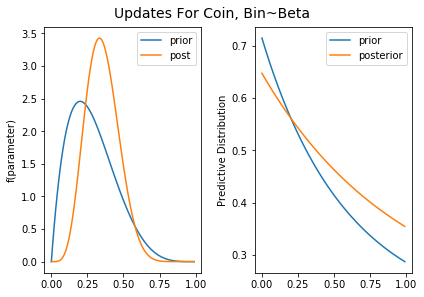
\includegraphics[width=1\textwidth]{update_param_pred.png}
\caption{\label{Updating parameter and likelihood} From the 'hub.}
\end{figure}
\fi

\subsection{Prior Predictive Function}
In the coin case we started assuming nothing about the coin. What does this lead us to expect for each value of the observable in $\{0,1,2,...,20 \}$? Just considering the likelihood, we can answer this question \textit{for a particular choice of $\theta$}, but now we integrate out the parameter.
The general form is
\begin{equation}
    f(x) = \int_\theta f(x|\theta)f(\theta)\ d\theta,
\end{equation}
and in this case it is
\begin{equation}
    f(x) = \int_{0}^{1} {\frac{20!}{x!(20-x)!}} \theta^x (1-\theta)^{20-x}.
\end{equation}
While you could do that integral the direct way, I suggest side-stepping it by spotting it is nearly a Beta distribution, with $\alpha=x+1$ and $\beta=20-x+1$, and therefore $\alpha+\beta=22$.
\begin{equation}
    f(x) = \int_{0}^{1} {\frac{\Gamma(21)}{\Gamma(x+1) \Gamma(21-x))}} \theta^{(x+1)-1} (1-\theta)^{(21-x)-1} d\theta.
\end{equation}

The integrand would be the Beta distribution if the numerator of the combinatorial factor were $\Gamma(22)$, which is $21!$, so we multiply and divide by 21, giving
\begin{equation}
    f(x) = \frac{1}{21}\int_{0}^{1} {\frac{\Gamma(22)}{\Gamma(x+1) \Gamma(21-x))}} \theta^{(x+1)-1} (1-\theta)^{(20-x)-1}
    = \frac{1}{21}.
\end{equation}

There was nothing special about $21$ here, it is simply the size of the observable set in the Binomial likelihood, ie $n+1$. What we have shown is that a uniform prior leads to to a uniform predictive distribution. This is not surprising if you consider that for every distribution with a small $\theta$, say $0.1$, there is one with a large one, here $0.9$, and $\theta$ is just as likely to take either value. In summary, the distribution of the number of Binomial successes averaged out over all the possible parameter values (at their respective probabilities, and using discrete-distribution language) is simply

\begin{equation}
    p(X=0)=p(X=1)=p(X=2)=...=p(X=20)=\frac{1}{21}. \label{predictive_unif}
\end{equation}

\begin{Exercise}
    \paragraph{Concept checker: discrete prior} In the context of a hospital with $20$ patients with coronavirus interested in predicting how many might need to transferred to the ICU, suppose the medics apply their collective expertise to conclude there are two candidates for the way the disease will behave. In one case, which is the most likely, at $90\%$, $\theta=0.3$; but in the other, more serious but unlikely case, $\theta=0.9$. What is the probability that $20$ patients need intensive care? How does this compare to the answer if we assume $\theta=0.3$? What if they only have capacity for ten in their ICU?
    
    \paragraph{Hint} Draw a tree where the first split represents the possibilities for $theta$ and the second the observable. This is discrete so you are not integrating, just taking a weighted average (ie applying Bayes' formula). The outlook worsens considerably.
\end{Exercise}

\subsection{Posterior Predictive Function}
Again we integrate out the parameter but use the data as well as the prior, by replacing $f(\theta)$ with its updated version having observed data, $f(\theta|d)$. A more algebraic approach to see why this gives what we want is to use the Chain Rule and then the independence of future observations from past ones:
\begin{equation}
\begin{split}
        f(x|d) 
        &= \int_\theta f(x|d,\theta)f(\theta|d)\ d\theta \\
        &= \int_\theta f(x|\theta)f(\theta|d)\ d\theta \\
\end{split}
\end{equation}

Note that the integrand is the product of the likelihood and the current distribution for the parameter, just like with the prior predictive function, but the current distribution has changed from the prior to the posterior.


\subsubsection{Beta-Binomial Distribution}
For a Beta prior and Binomial likelihood, the predictive function takes on the form of a Beta-Binomial distribution - see equation \eqref{betabinomial} below.

\begin{Exercise}
    \paragraph{Consolidatory Exercise} Find the predictive distirbution for the second flip given the first was Heads. That is, find $f(X_2=0|X_1=1)$ and $f(X_2=1|X_1=1)$.
    
    \paragraph{Hint} Find the integral form. Do not integrate directly. Rather spot that your integral can be split into the difference of two integrals one of which is simply an entire density function and the other is an expectation, for which you have a formula. Confirm your answers by direct integration.'
\end{Exercise}

\begin{Exercise}
    \paragraph{Consolidatory Exercise}
    Prove that the general form of the (prior or posterior) predictive function for a Beta$(\alpha, \beta)$ prior and Binomial$(n,\theta)$ likelihood is Beta-Binomial, ie  
    \begin{equation}
        f(x)=\frac{\Gamma(n+1)}{\Gamma(x+1)\Gamma(n-x+1)}
        \frac{\Gamma(x+\alpha)\Gamma(n-x+\beta)}{\Gamma(n+\alpha+\beta)}
        \frac{\Gamma(\alpha+\beta)}{\Gamma(\alpha)\Gamma(\beta)}.
        \label{betabinomial}
    \end{equation}
    
    \paragraph{Hint}
    It is easy if you use the spotting trick; your integral is a constant times something which is a Beta distribution missing its combinatorial factor; insert it and you're done.
\end{Exercise}

\begin{Exercise}
    \paragraph{Consolidatory Exercise} Prove that the equation above \eqref{betabinomial} reduces to the discrete Uniform distribution in the prior case that $(\alpha,\beta)=(1,1)$, in agreement with equation \eqref{predictive_unif}.
    
    \paragraph{Hint}
    Substituting ones for both parameters simplifies that fraction to $\frac{1}{n+1}$, for any $x$.
\end{Exercise}

\subsection{Poisson Likelihood and Gamma Prior}

\begin{Exercise}
\paragraph{Exploration Assignment}
    Deduce as much as you can about the form of the predictive function. If you use 'specialisation and generalisation', begin with a single observation.
\end{Exercise}

\subsection{Exponential Likelihood and Gamma Prior}

\begin{Exercise}
\paragraph{Exploration Assignment}
    Deduce as much as you can about the form of the predictive function. If you use 'specialisation and generalisation', begin with a single observation.
\end{Exercise}

\section{Credibility Intervals}
These are what students think they're learning when they first come across confidence intervals: the probability that the parameter lies in an interval. Common uses are Equal-Tail, eg the central 10\%, and Highest Density, such as the narrowest interval containing 10\% (which will always contain the mode). Rather than integrate directly, it is preferable to use quantile functions in a stats-friendly programming language like R.

Continuing with the (f)unfair coin example, suppose we want to know how the probability of the coin's being roughly fair evolves, as well as the chance that it is very unfair. Let's choose corresponding $\theta$ intervals as $[0.4,0.6]$ and $[0,0.1]\cup[0.9,1]$ respectively.

\paragraph{Prior Intervals}
\begin{equation}
    p(\theta \in[0.4,0.6])=\int_{0.4}^{0.6} 1 \ d \theta = 0.2
\end{equation}

\begin{equation}
    p(\theta \in[0,0.1]\cup[0.9,1])=\int_{0}^{0.1} 1 \ d \theta +\int_{0.9}^{1} 1 \ d \theta = 0.2
\end{equation}

\begin{Exercise}
    \paragraph{Consolidation Exercise}
    Find the equivalent probabilities for the next few iterations, and any other probabilities you find interesting. For example, the deciles.
\end{Exercise}

\paragraph{Fixed Probability Intervals}
Where Frequentist statistics uses confidence intervals around an observation to express a statement about the observation in relation to $\mu$, the Bayesian paradigm offers credible intervals making statements about $\mu$ given the observation, and typical forms include equal tailed intervals (the probability of the parameter lying below is the same as its falling above the interval) and highest density intervals (the narrowest interval of a given area).

To illustrate, consider the funfair coin. Suppose we start out with a uniform distribution for $\theta$ (Beta(1,1)) and then observe 14 Heads out of 18 flips; then the posterior is Beta(15,5), suggesting the coin is Heads-heavy. We calculate $89\%$ intervals both ways using R:

\begin{itemize}

\item \text{HDI: [0.81, 0.99]} 
\item \text{ETI: [0.78, 0.98]} 
.
\end{itemize}

\begin{figure}[h]
\centering
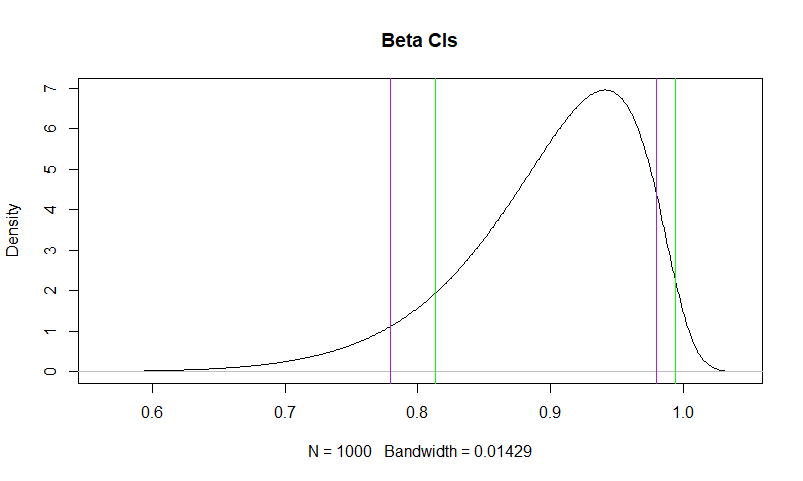
\includegraphics[width=1.0\textwidth]{Beta_CIs.png}
\caption{\label{fig:Beta_CIs} HDI in green, ETI in purple}
\end{figure}
\newpage

\section{Markov Chain Monte Carlo (MCMC)}
What happens when, as in the majority of cases, the prior is not conjugate to the likelihood? Usually the posterior involves a normalising constant that is an intractable integral. For example a Normal likelihood with known variance and a t-Distribution for the mean. One approach is to use computational approximations for the posterior, and the most used is MCMC. This uses a Markov Chain whose stationary distribution is precisely the posterior distribution, and so iterating can approximate it with arbitrary precision.

\begin{Exercise}
    Estimate the geometric constant $\pi$ by generating bivariate uniform pairs $(x,y)$ each on $[-1,1]$ and using the proportion of them inside a unit circle.
\end{Exercise}

\subsection{Metropolis-Hastings (cf Quantum MH)}
The most used MCMC is Bayesian estimation. The algorithm aims to simulate the target distribution by drawing candidates from some proposal distribution and accepting those that are plausible enough.

Suppose you want posterior $p$ but only know $g$, where $p \propto g$. Let $q$ be the proposal distribution.

\begin{algorithm}[H]
\SetAlgoLined
\KwResult{A set of points consistent with target posterior distribution}
 initialise $\theta_0$\;
 \For{i in 1:m }{
  generate candidate $\theta^{*}$ from $q(\theta^{*}|\theta_{i-1})$\;
  calculate acceptance rate $\alpha$; \\
  accept $\theta^{*}$ with probability $\alpha$, so  \\
  \eIf{accept candidate}{
   $\theta_{i} := \theta^{*}$\;
   }{
   $\theta_{i} := \theta_{i-1}$\;
  }
 }
 \caption{Metropolis-Hastings}
 
 Note that the acceptance rate is
 
 \begin{equation}
    \alpha=\min{(1, \frac{g(\theta^{*})}{g(\theta_{i-1})}
    \frac{q(\theta_{i-1}|\theta^{*})}{q(\theta^{*}|\theta_{i-1})})}   .
 \end{equation}
 
\end{algorithm}

The first fraction, $\frac{g(\theta^{*})}{g(\theta_{i-1})}$, promotes candidates that are more likely than the previous one, so pushes the simulation up the desired PDF. The second one, $\frac{q(\theta_{i-1}|\theta^{*})}{q(\theta^{*}|\theta_{i-1})}$, promotes exploration which is crucial in multi-modal target distributions, for example; it acts against any tendency to get stuck.

\section{Glossary}
\paragraph{Caveat}
Regarding the use of indicator functions or explicit statements about ranges where a function is obviously zero outside a particular interval, the advantages in the unlikely case of ambiguity seem outweighed by the disadvantages of visual clutter, so I have generally used these things sparingly. For example, if a distribution is 1 on [0,1] and 0 elsewhere, I may just point out that it is 1 on [0,1] and leave the rest implicit.
\section{Select Omissions}
How to choose prior (effective sample size, mean, variance, informativeness etc)

\end{document}

R metro hast

lg = function(mu, n, ybar) {
  mu2 = mu^2
  n * (ybar * mu - mu2 / 2.0) - log(1 + mu2)
}

mh = function(n, ybar, n_iter, mu_init, cand_sd) {
  ## Random-Walk Metropolis-Hastings algorithm
  
  ## step 1, initialize
  mu_out = numeric(n_iter)
  accpt = 0
  mu_now = mu_init
  lg_now = lg(mu=mu_now, n=n, ybar=ybar)
  
  ## step 2, iterate
  for (i in 1:n_iter) {
    ## step 2a
    mu_cand = rnorm(n=1, mean=mu_now, sd=cand_sd) # draw a candidate
    
    ## step 2b
    lg_cand = lg(mu=mu_cand, n=n, ybar=ybar) # evaluate log of g with the candidate
    lalpha = lg_cand - lg_now # log of acceptance ratio
    alpha = exp(lalpha)
    
    ## step 2c
    u = runif(1) # draw a uniform variable which will be less than alpha with probability min(1, alpha)
    if (u < alpha) { # then accept the candidate
      mu_now = mu_cand
      accpt = accpt + 1 # to keep track of acceptance
      lg_now = lg_cand
    }
    
    ## collect results
    mu_out[i] = mu_now # save this iteration's value of mu
  }
  
  ## return a list of output
  list(mu=mu_out, accpt=accpt/n_iter)
}

y = c(1.2, 1.4, -0.5, 0.3, 0.9, 2.3, 1.0, 0.1, 1.3, 1.9)
ybar = mean(y)
n = length(y)
hist(y, freq=FALSE, xlim=c(-1.0, 3.0)) # histogram of the data
curve(dt(x=x, df=1), lty=2, add=TRUE) # prior for mu
points(y, rep(0,n), pch=1) # individual data points
points(ybar, 0, pch=19) # sample mean

set.seed(43) # set the random seed for reproducibility
post = mh(n=n, ybar=ybar, n_iter=1e3, mu_init=0.0, cand_sd=3.0)
str(post)

library("coda")
traceplot(as.mcmc(post$mu))

post = mh(n=n, ybar=ybar, n_iter=1e3, mu_init=0.0, cand_sd=0.05)
post$accpt

traceplot(as.mcmc(post$mu))

post = mh(n=n, ybar=ybar, n_iter=1e3, mu_init=0.0, cand_sd=0.9)
post$accpt

traceplot(as.mcmc(post$mu))

post = mh(n=n, ybar=ybar, n_iter=1e3, mu_init=30.0, cand_sd=0.9)
post$accpt

traceplot(as.mcmc(post$mu))

post$mu_keep = post$mu[-c(1:100)] # discard the first 200 samples
plot(density(post$mu_keep, adjust=2.0), main="", xlim=c(-1.0, 3.0), xlab=expression(mu)) # plot density estimate of the posterior
curve(dt(x=x, df=1), lty=2, add=TRUE) # prior for mu
points(ybar, 0, pch=19) # sample mean

curve(0.017*exp(lg(mu=x, n=n, ybar=ybar)), from=-1.0, to=3.0, add=TRUE, col="blue") # approximation to the true posterior in blue

